%%
%% This is file `mcmthesis-demo.tex',
%% generated with the docstrip utility.
%%
%% The original source files were:
%%
%% mcmthesis.dtx  (with options: `demo')
%% 
%% -----------------------------------
%% 
%% This is a generated file.
%% 
%% Copyright (C)
%%     2010 -- 2015 by Zhaoli Wang
%%     2014 -- 2016 by Liam Huang
%% 
%% This work may be distributed and/or modified under the
%% conditions of the LaTeX Project Public License, either version 1.3
%% of this license or (at your option) any later version.
%% The latest version of this license is in
%%   http://www.latex-project.org/lppl.txt
%% and version 1.3 or later is part of all distributions of LaTeX
%% version 2005/12/01 or later.
%% 
%% This work has the LPPL maintenance status `maintained'.
%% 
%% The Current Maintainer of this work is Liam Huang.
%% 
\documentclass{mcmthesis}
\mcmsetup{CTeX = false,   % 使用 CTeX 套装时,设置为 true 
        tcn = 82104, problem = C,
        sheet = true, titleinsheet = true, keywordsinsheet = true,
        titlepage = false, abstract = true}
\usepackage{palatino}
\usepackage{subfig}
\usepackage[font=footnotesize,labelfont=bf]{caption}
\usepackage[retainorgcmds]{IEEEtrantools}
\usepackage{tabularx}
\usepackage{setspace}
\usepackage{calc}

\makeatletter
\newcommand{\DESCRIPTION@original@item}{}
\let\DESCRIPTION@original@item\item
\newcommand*{\DESCRIPTION@envir}{DESCRIPTION}
\newlength{\DESCRIPTION@totalleftmargin}
\newlength{\DESCRIPTION@linewidth}
\newcommand{\DESCRIPTION@makelabel}[1]{\llap{#1}}%
\newcommand{\DESCRIPTION@item}[1][]{%
  \setlength{\@totalleftmargin}%
       {\DESCRIPTION@totalleftmargin+\widthof{\textbf{#1 }}-\leftmargin}%
  \setlength{\linewidth}
       {\DESCRIPTION@linewidth-\widthof{\textbf{#1 }}+\leftmargin}%
  \par\parshape \@ne \@totalleftmargin \linewidth
  \DESCRIPTION@original@item[\textbf{#1}]%
}
\newenvironment{DESCRIPTION}
  {\list{}{\setlength{\labelwidth}{0cm}%
           \let\makelabel\DESCRIPTION@makelabel}%
   \setlength{\DESCRIPTION@totalleftmargin}{\@totalleftmargin}%
   \setlength{\DESCRIPTION@linewidth}{\linewidth}%
   \renewcommand{\item}{\ifx\@currenvir\DESCRIPTION@envir
                           \expandafter\DESCRIPTION@item
                        \else
                           \expandafter\DESCRIPTION@original@item
                        \fi}}
  {\endlist}
\makeatother

\title{Energy production}
\author{\small \href{http://www.latexstudio.net/}
  {
\includegraphics[width=7cm]{mcmthesis-logo}}}
\date{\today}
\begin{document}
\begin{abstract}
Energy problem has always been a great concern for the U.S.
Nowadays, it is urgent to strengthen cooperation between states, since a single state cannot achieve the optimal goals without others' assistance.
The four states of America boarding with Mexico are going to reach an interstate compact on energy policy, and our work is to build mathematical models with historical data to set targets for the four states and to list some actions which can be taken by the governors.

For part I, firstly, in order to create an energy profile of each state, we pick some key variables to summarize the energy usage from the massive historical data.
More specifically, we focus on the production and consumption of major conventional and renewable energy sources, and then picture them separately to give a vivid view.
Secondly, we use XGBoost algorithm to create an energy index named $W$, which represents the comprehensive use of energy in each state.
The evolution is shown clearly in the diagrams.
Then we apply the same algorithm to renewable energy sources to describe their usage.
Combined with other factors such as geography, population and climate, we give a further discussion about the energy profile of cleaner, renewable energy usage.
Thirdly, we extract the data of major renewable energy sources of the four states in 2009, and applied Topsis method to determine the best energy profile for use of cleaner energy.
Finally, we use the Prophet Forecasting Model to predict the energy profile of each state in 2025 and 2050, in which we introduce seasonality (financial crisis) to make the prediction more accurate and convincing.

For part II, we summarize the results of our models and set energy targets for the four states in the interstate compact.
Furthermore, we give feasible advice for the governors on how to achieve these goals.

Of course, there are some defects in our model, but it will be more effective and practical with further studies.

\begin{keywords}
XGBoost, Topsis, Prophet, Time Series, Seasonality
\end{keywords}
\end{abstract}
\maketitle
\tableofcontents
\newpage


\section{Introduction}
\subsection{Background}
While industrialization boosts productivity significantly, it also calls for a huge amount of resources, including energy.
In fact, any industrialized body would be very fragile without a robust energy supplying system.
Thus, among all the factors, energy production and usage has become one of the most vital aspects of an economy.

In the United States, without a centralized energy management department, energy policies are left to state governments to decide, which does make some sense considering the different features of every state.
However, we cannot get the global optimum without many close interstate cooperations, but the decentralization of decision-making power makes this goal harder to achieve.

As an attempt to address this issue, the Western Interstate Energy Compact (WIEC) was formed in 1970 by twelve western states, aiming to foster cooperation between these states for the development and management of nuclear energy technologies.
Thanks to WIEC, interstate cooperations are now easier with interstate compacts, which are contractual arrangements made between two or more states. These compacts are based on a specific policy issue and put into force either the adoption of a set of standards or the cooperation within these states on a particular regional or national matter.


\section{Analysis of the Problem and Our Work}
California, Arizona, New Mexico and Texas are four states standing in the transition stage of energy sources. Some of them have good conditions of exploiting cleaner, renewable energy sources, while others are in need of energy supplement or technological assistance. In the interstate compact, the utility of every resource ought to be maximized, which is our fundamental goal. 

\subsection{Part I}
\begin{DESCRIPTION}
\item [A] Plentiful variables related to energy usage in four states are given in the data file, which calls for careful selection to reveal the specific energy profile of these states.
Each type of energy is depicted in two aspects, production and consumption.
The former might be detailed to the five sectors, that is transportation sector, commercial sector, industrial sector, residential sector and electric power sector, while the latter is mostly depicted in some macroscopic factors.
Of course, the absence of certain data is a tough problem when choosing the factors we need.

After analysis, we decide to depict the energy profile in three different ways:
\begin{itemize}  
\item Consumption in different sectors, varying from 1960 to 2009 in four states.
\item Production of several major conventional energy source, varying from 1960 to 2009 in four states. 
\item Price of these energy source and the total average price, varying from 1960 to 2009 in four states.
\end{itemize}

\item [B] To characterize how energy profile of four states evolve from 1960 to 2009, we need to summarize the variables we choose and try to get an energy index $W$, representing integrated energy profile.
To achieve this, we use XGBoost algorithm, and conduct more data analysis on the results, which turns out to be satisfying to some extent.

In order to inspect the usage of cleaner, renewable energy resources in the four states, we need to detail this part in our model, and analyze several important renewable energy sources further.
The different orientation of utilizing renewable energy sources may be caused by the factors specific to a state, like geography, climate and population.
Consequently, more information about the four states is required.
With diagrams illustrating the similarities and differences between four states, the outcomes become more explicit.

\item [C] One of the four states has the best energy profile for using renewable energy resources.
An evaluation method is required to decide which one is the best.
Topsis algorithm is the easiest and most effective way to do that.

\item [D] Prediction is the vital part of the model, directly connecting to the goals of the intestate compact.
Time series analysis can do that perfectly. 
Through the production, we also take some other potential factors into consideration, which will make our prediction more accurate.
\end{DESCRIPTION}

\subsection{Part II}
\begin{DESCRIPTION}

\item [A] By summarizing our work in Part I, we need to further discuss the targets of renewable energy sources in 2025 and 2050, and formally state them in the interstate compact of the four states.

\item [B] The goals of the energy usage cannot be achieved without the four states' contribution and cooperation.
Therefore, recommendation about several feasible actions is made.
\end{DESCRIPTION}

\subsection{Part III}
We summarize our work in the former two parts and recommend the goals in the compact, and then write a memo to the governors of the four states.

\section{Nomenclature}
See table~\ref{table:nomenclature}

\begin{table}[h]
\centering
\begin{tabular}{cc}
\hline Symbol & Definition \\ \hline
$Obj^{(t)}$ & the dependent variable of the objective function \\
$W$ & the comprehensive variable of energy profile \\
$RenewP$ & the proportion of renewable energy sources in production \\
$y(t)$ & the dependent variable of the prediction equation \\
$g(t)$ & the trend function representing the non-periodic changes \\
$s(t)$ & the trend function representing the periodic changes \\
$A$ & the data matrix of renewable energy usage \\
$B$ & the matrix $A$ normalized \\ 
$w$ & the weight of each energy resource in Topsis \\
$C$ & the matrix $B$ with weight on the variables \\
$S^{*}$ & the distance of each vector to the optimal solution \\
$S^{0}$ & the distance of each vector to the negative ideal solution \\
$f^{*}$ & the integrated index of renewable energy usage
\end{tabular}
\caption{Nomenclature}
\label{table:nomenclature}
\end{table}

\section{Energy Profile}
To illustrate the energy profile of each state, we analyze the data given in "ProblemCData.xlsx”, which contains plentiful data of consumption and production of diverse energy sources.
Some data lists are vital information of most frequently-used energy, such as natural gas, coal, motor gasoline, while others may be the renewable sources like geothermal energy and hydroelectricity.
Among these 605 variables collected by the official organization, we choose several of them that is significant to our study, and depict them in line charts or area plots based on the time series.
In this case, we want to demonstrate the variation tendency of energy usage in the four states, and briefly compare them for the sake of further studies.

Here we provide the energy profile for each state through data visualization.
For each of the four states, figure (a) depicts the energy consumed by various sectors; figure (b) shows the energy produced through different means; figure (c) demonstrates the trend of renewable energy usage.

\begin{figure}[!h]
   \subfloat[\label{ep-az-1}]{%
      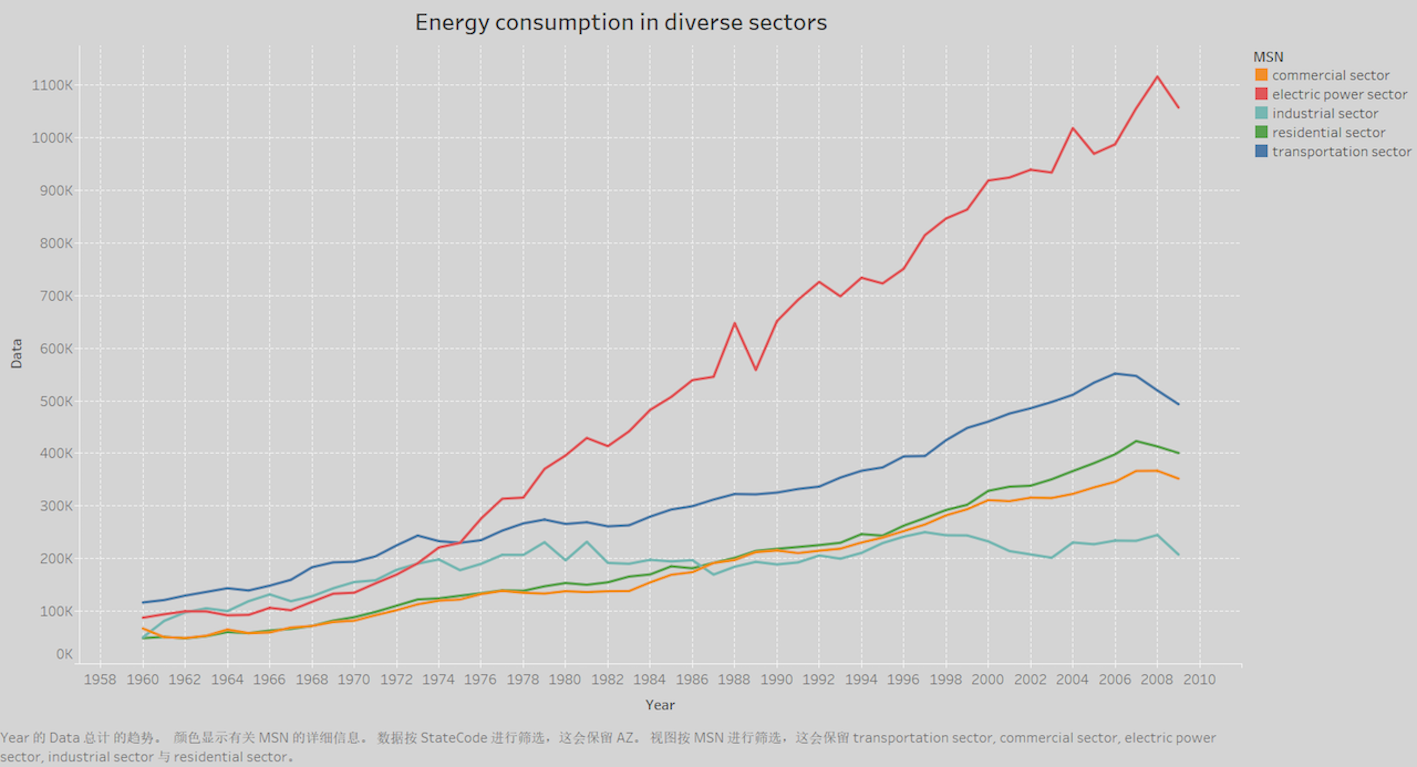
\includegraphics[width=0.3\textwidth]{ep/az-1.png}}
\hspace{\fill}
   \subfloat[\label{ep-az-2}]{%
      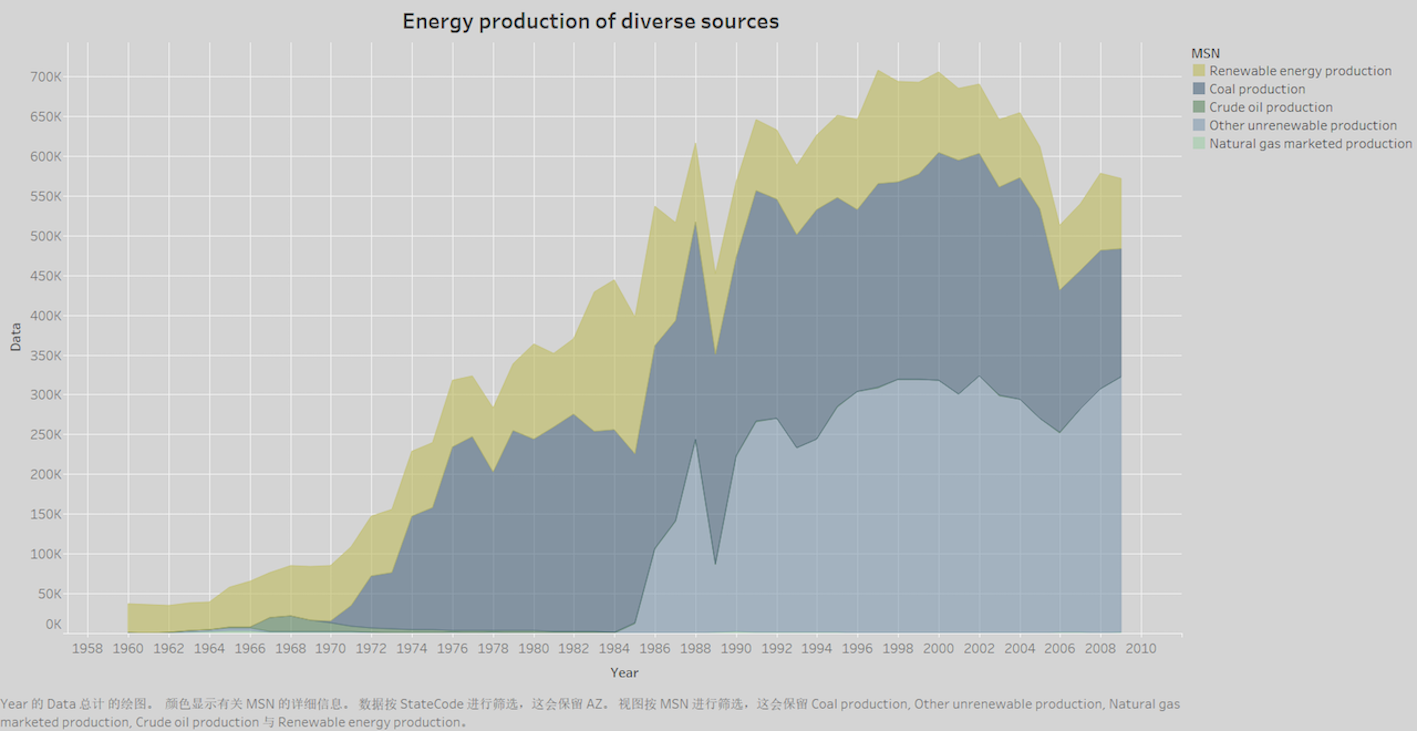
\includegraphics[width=0.313\textwidth]{ep/az-2.png}}
\hspace{\fill}
   \subfloat[\label{ep-az-3}]{%
      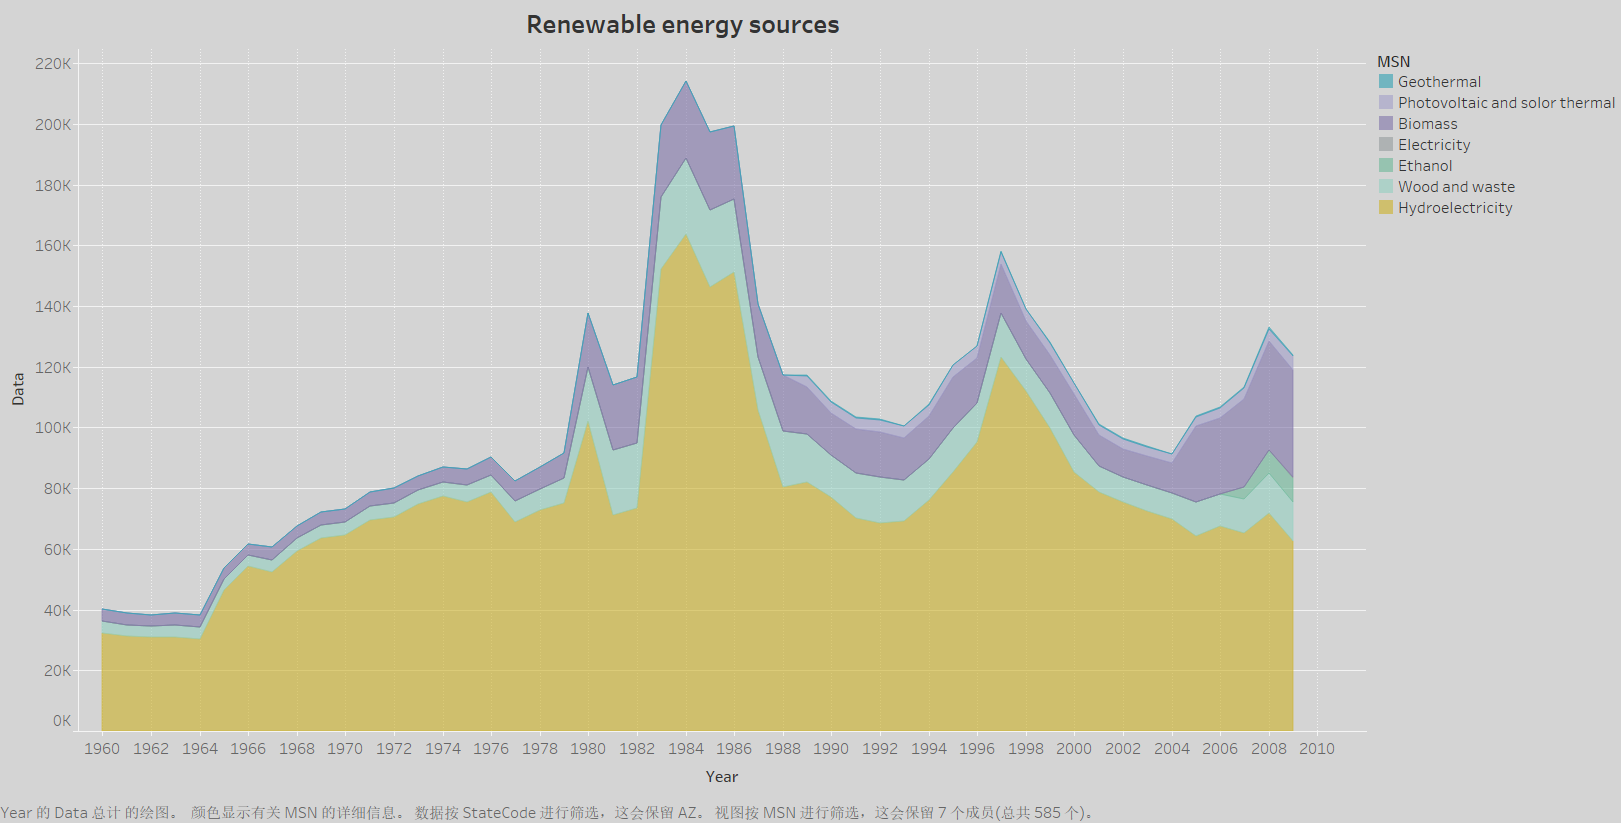
\includegraphics[width=0.32\textwidth]{ep/az-3.png}}
    \caption{The energy profile for Arizona (a) Energy consumption in diverse sectors (b) Energy production in diverse sources (c) Renewable energy usage}
    \label{fig:ep-az}
\end{figure}
\begin{figure}[!h]
   \subfloat[\label{ep-ca-1}]{%
      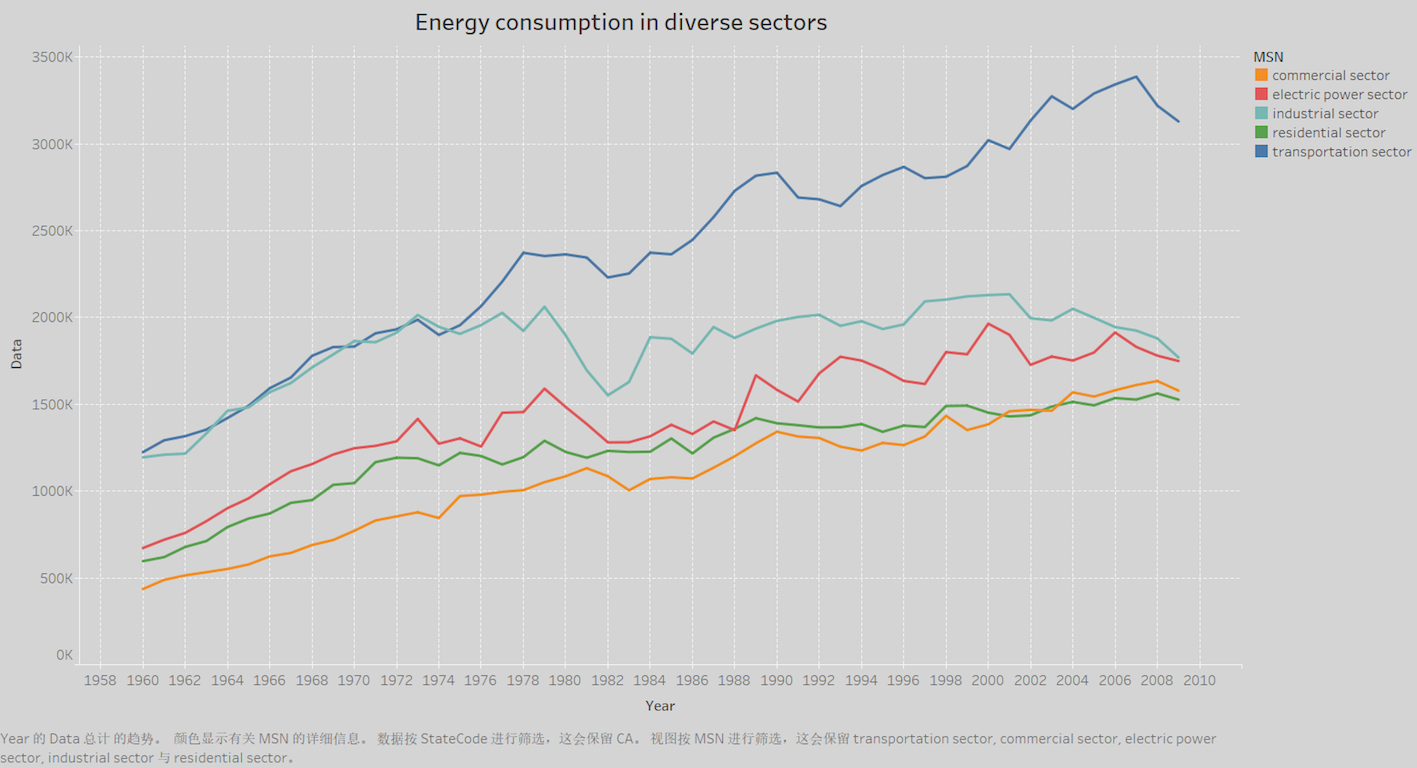
\includegraphics[width=0.3\textwidth]{ep/ca-1.png}}
\hspace{\fill}
   \subfloat[\label{ep-ca-2}]{%
      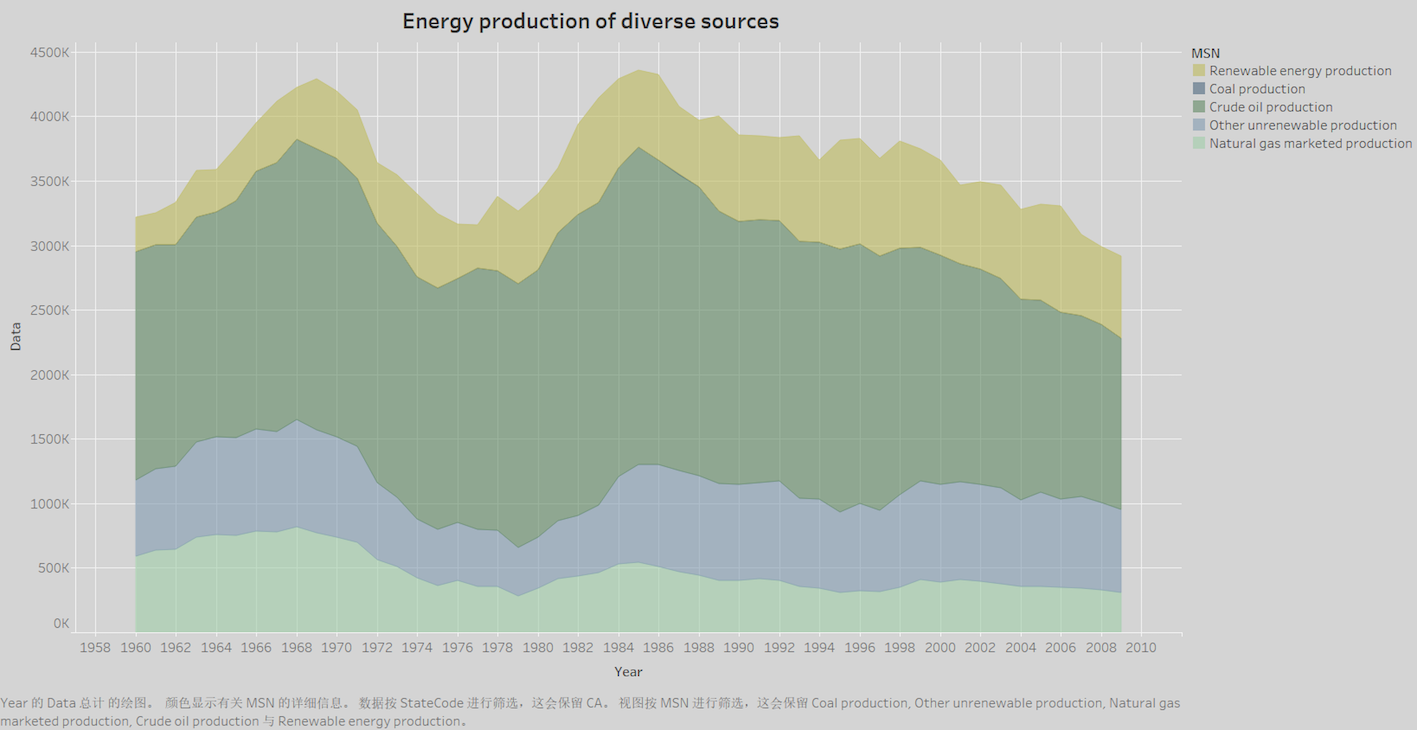
\includegraphics[width=0.313\textwidth]{ep/ca-2.png}}
\hspace{\fill}
   \subfloat[\label{ep-ca-3}]{%
      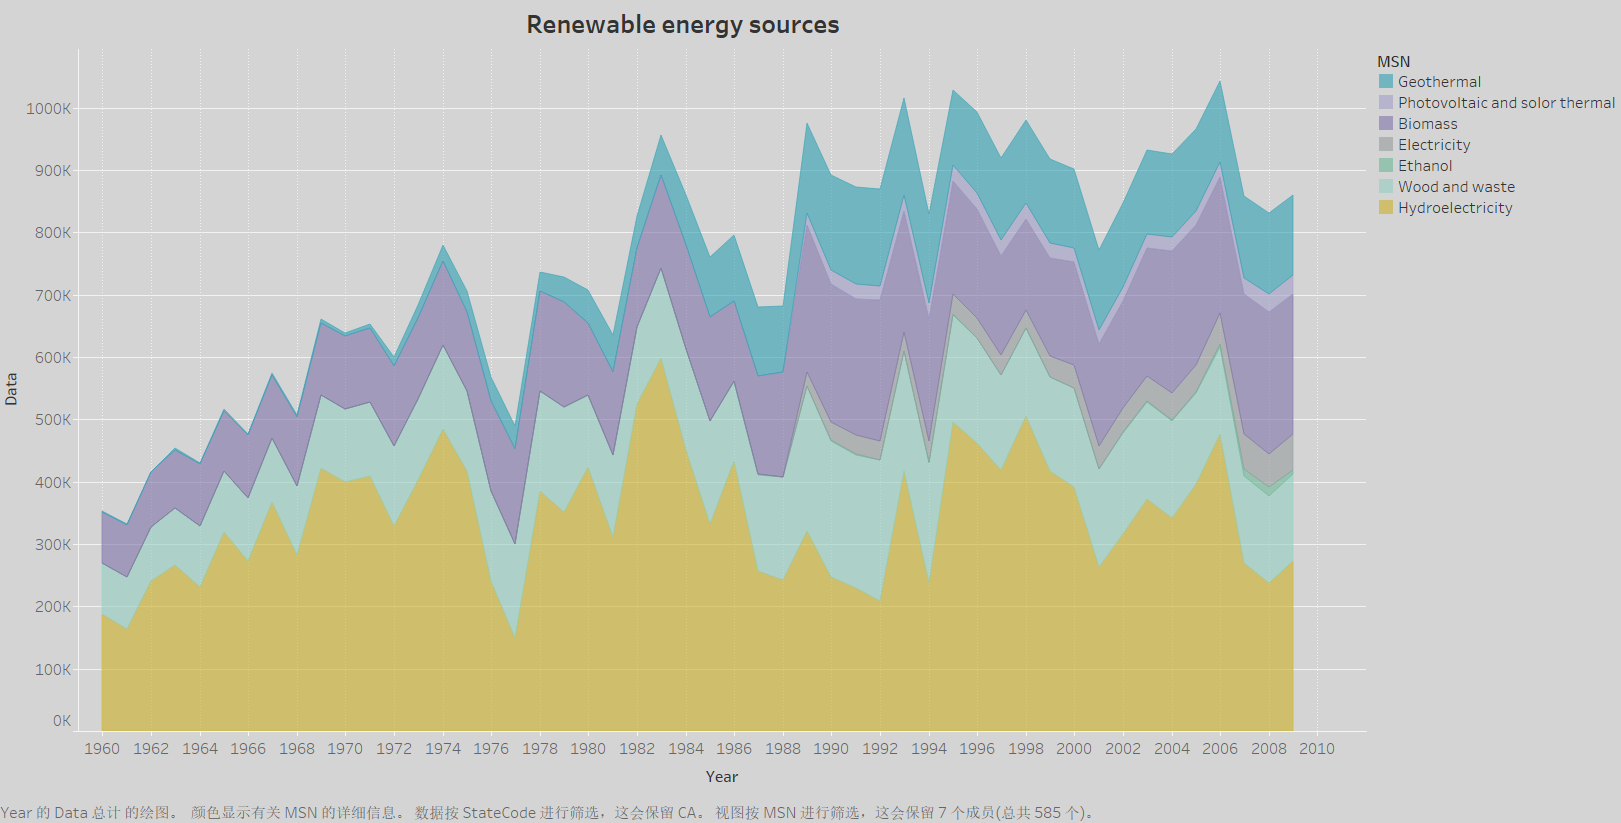
\includegraphics[width=0.32\textwidth]{ep/ca-3.png}}
    \caption{The energy profile for California (a) Energy consumption in diverse sectors (b) Energy production in diverse sources (c) Renewable energy usage}
    \label{fig:ep-ca}
\end{figure}
\begin{figure}[!h]
   \subfloat[\label{ep-nm-1}]{%
      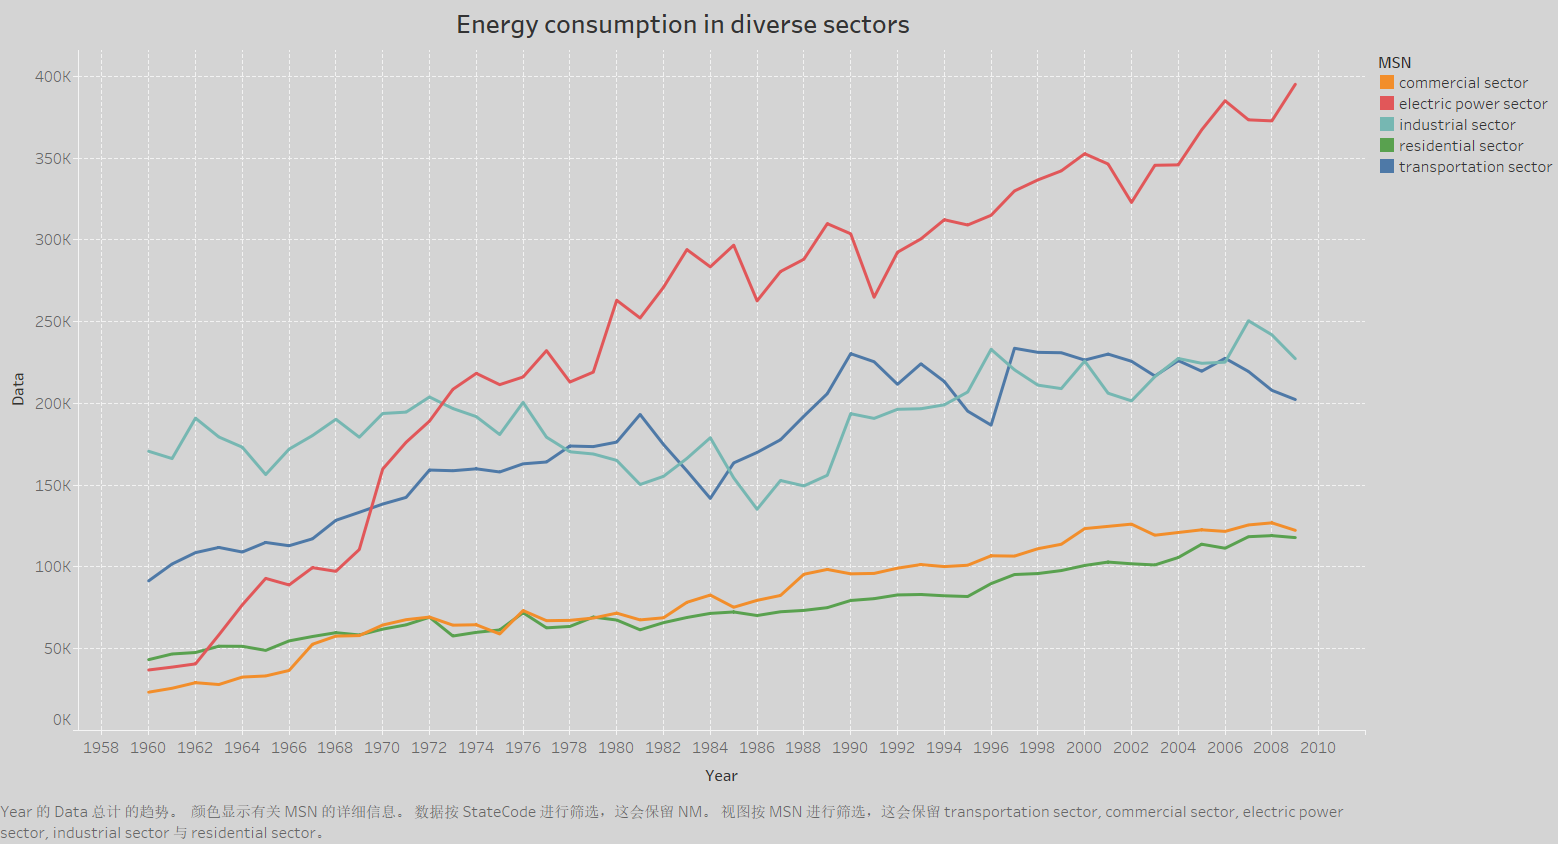
\includegraphics[width=0.3\textwidth]{ep/nm-1.png}}
\hspace{\fill}
   \subfloat[\label{ep-nm-2}]{%
      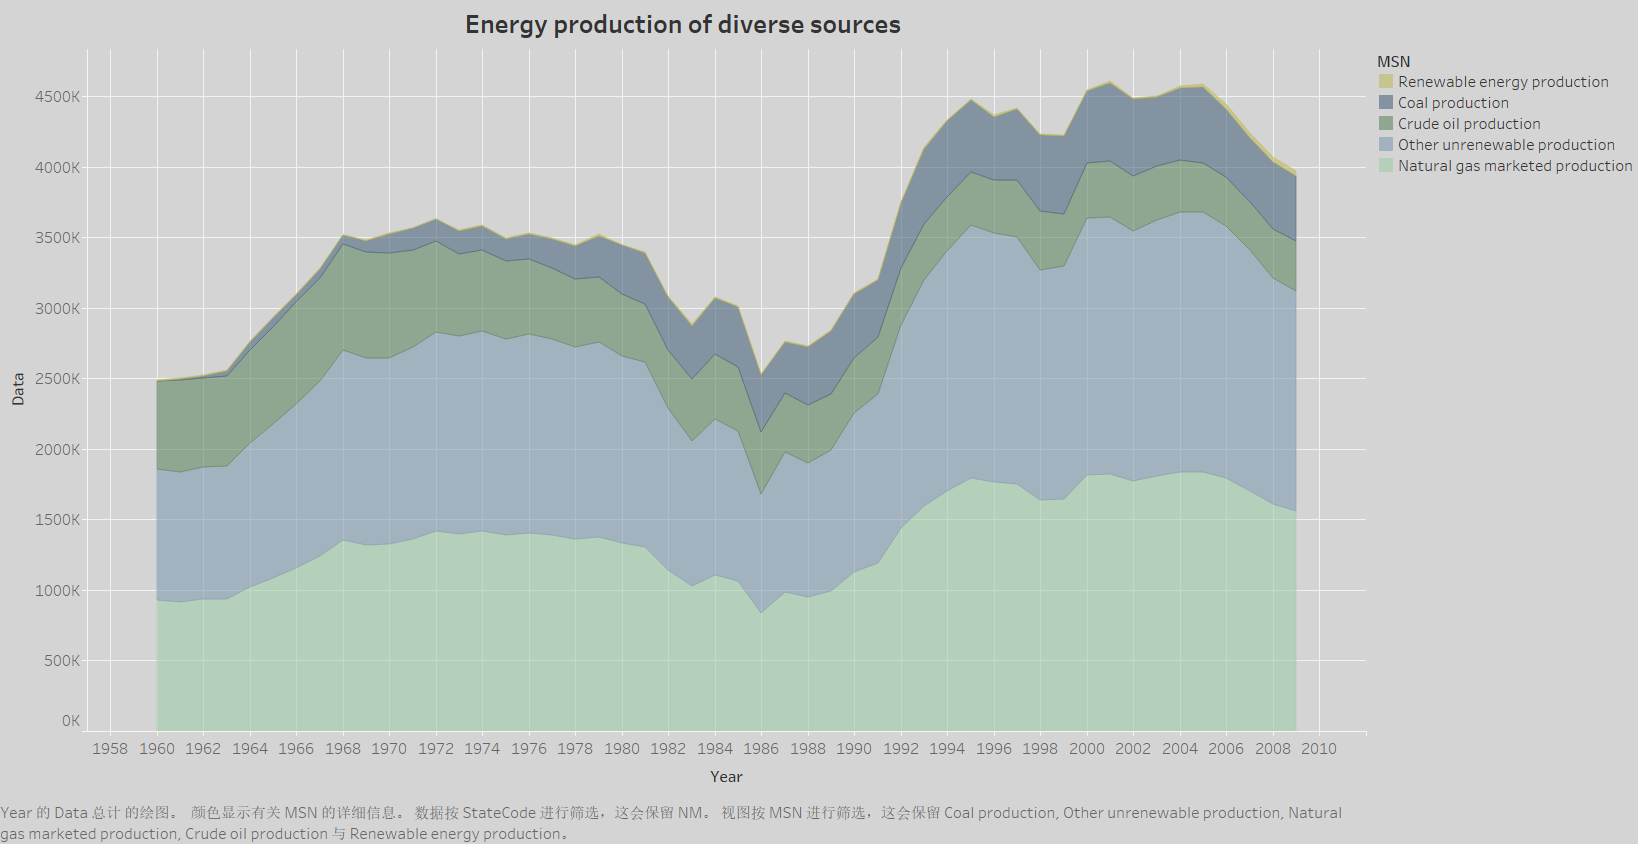
\includegraphics[width=0.313\textwidth]{ep/nm-2.png}}
\hspace{\fill}
   \subfloat[\label{ep-nm-3}]{%
      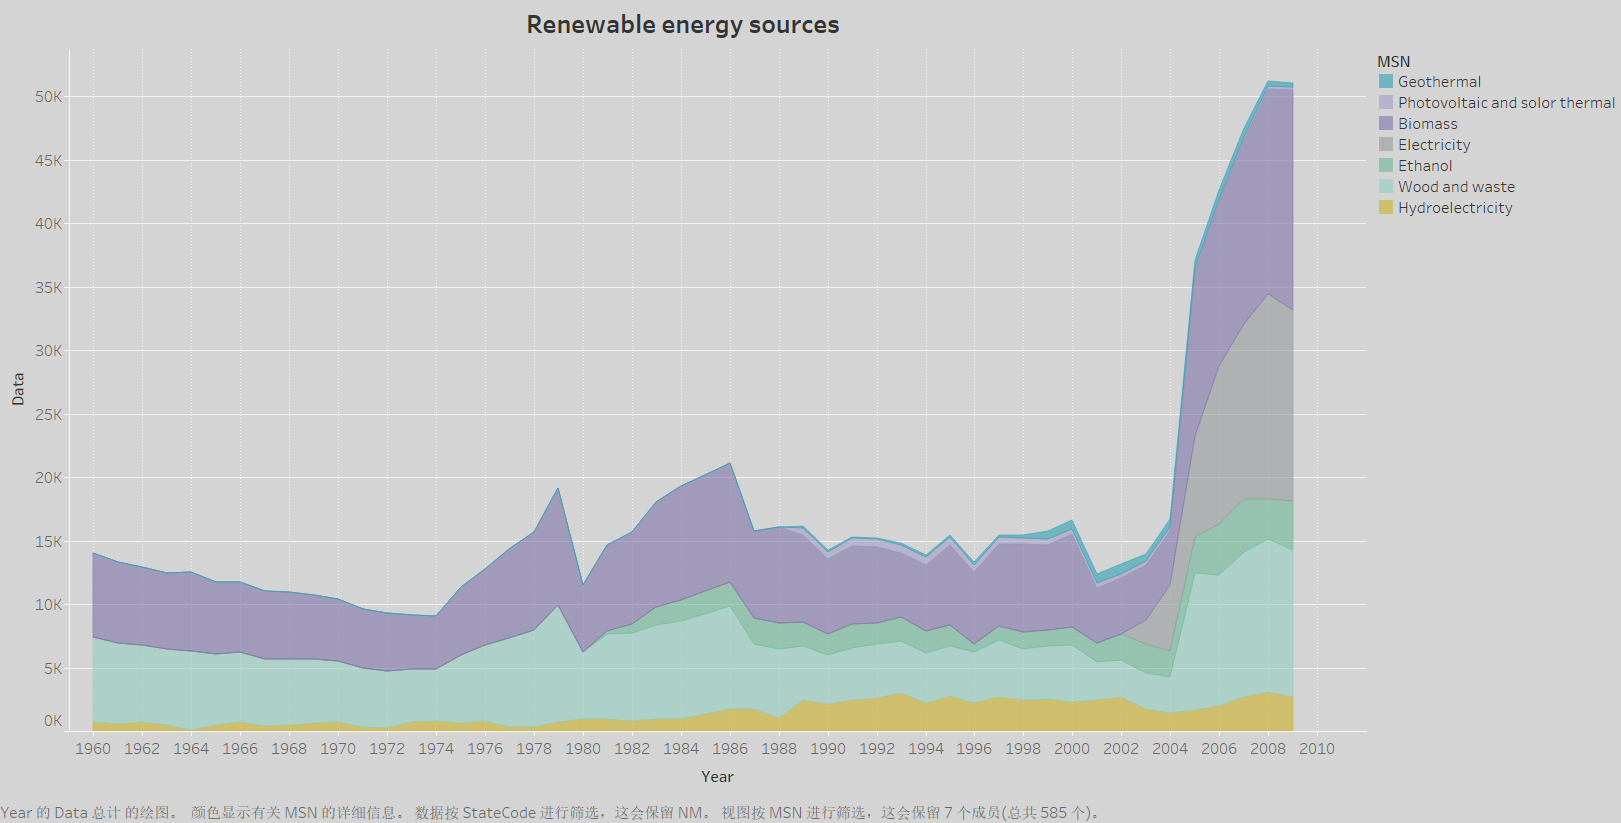
\includegraphics[width=0.32\textwidth]{ep/nm-3.png}}
    \caption{The energy profile for New Mexico (a) Energy consumption in diverse sectors (b) Energy production in diverse sources (c) Renewable energy usage}
    \label{fig:ep-nm}
\end{figure}
\begin{figure}[!h]
   \subfloat[\label{ep-tx-1}]{%
      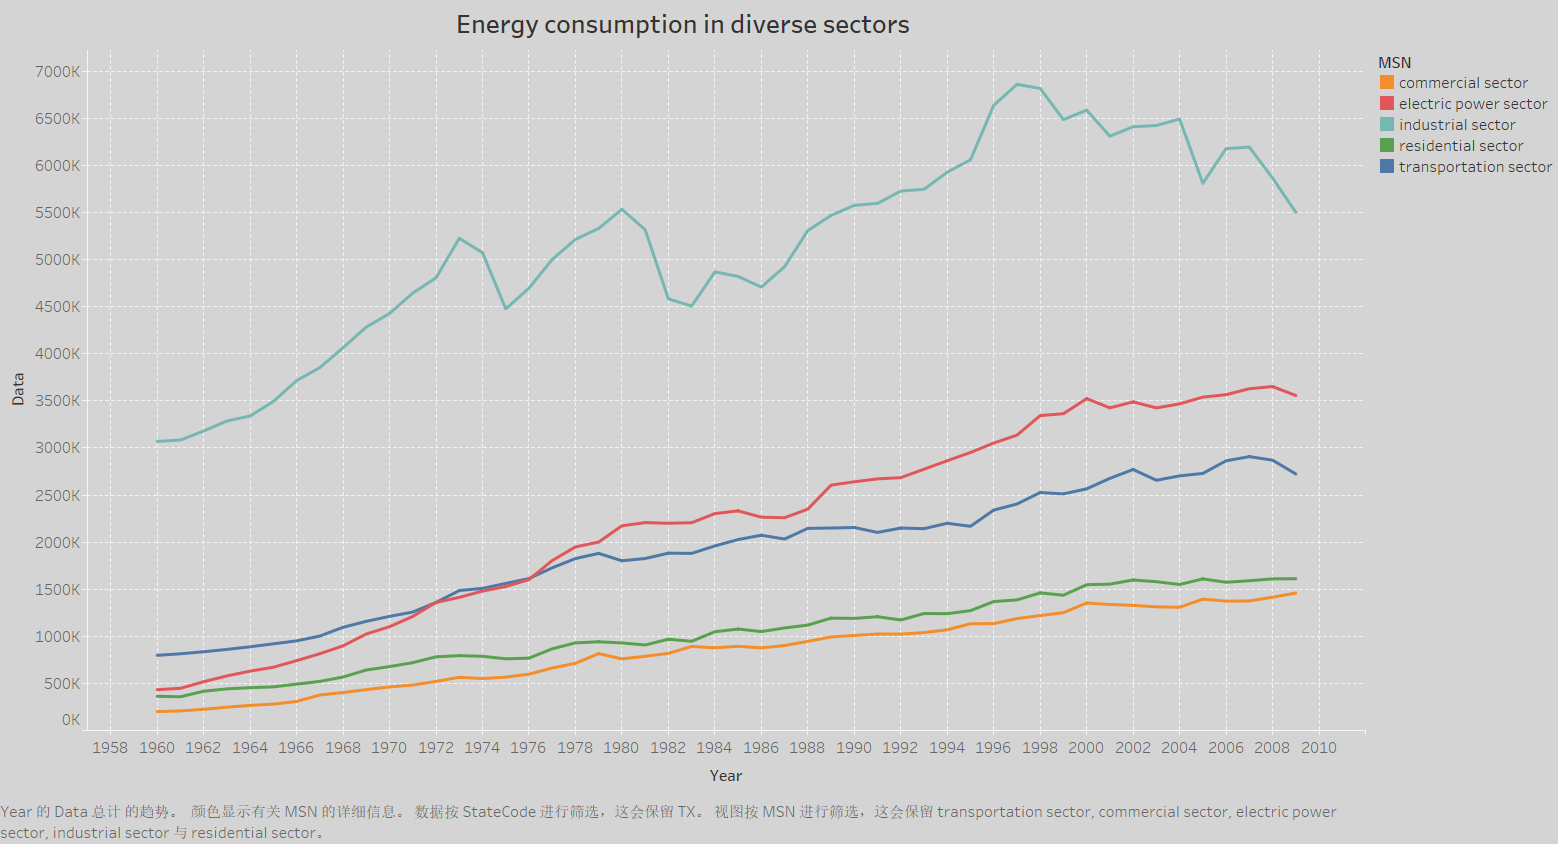
\includegraphics[width=0.3\textwidth]{ep/tx-1.png}}
\hspace{\fill}
   \subfloat[\label{ep-tx-2}]{%
      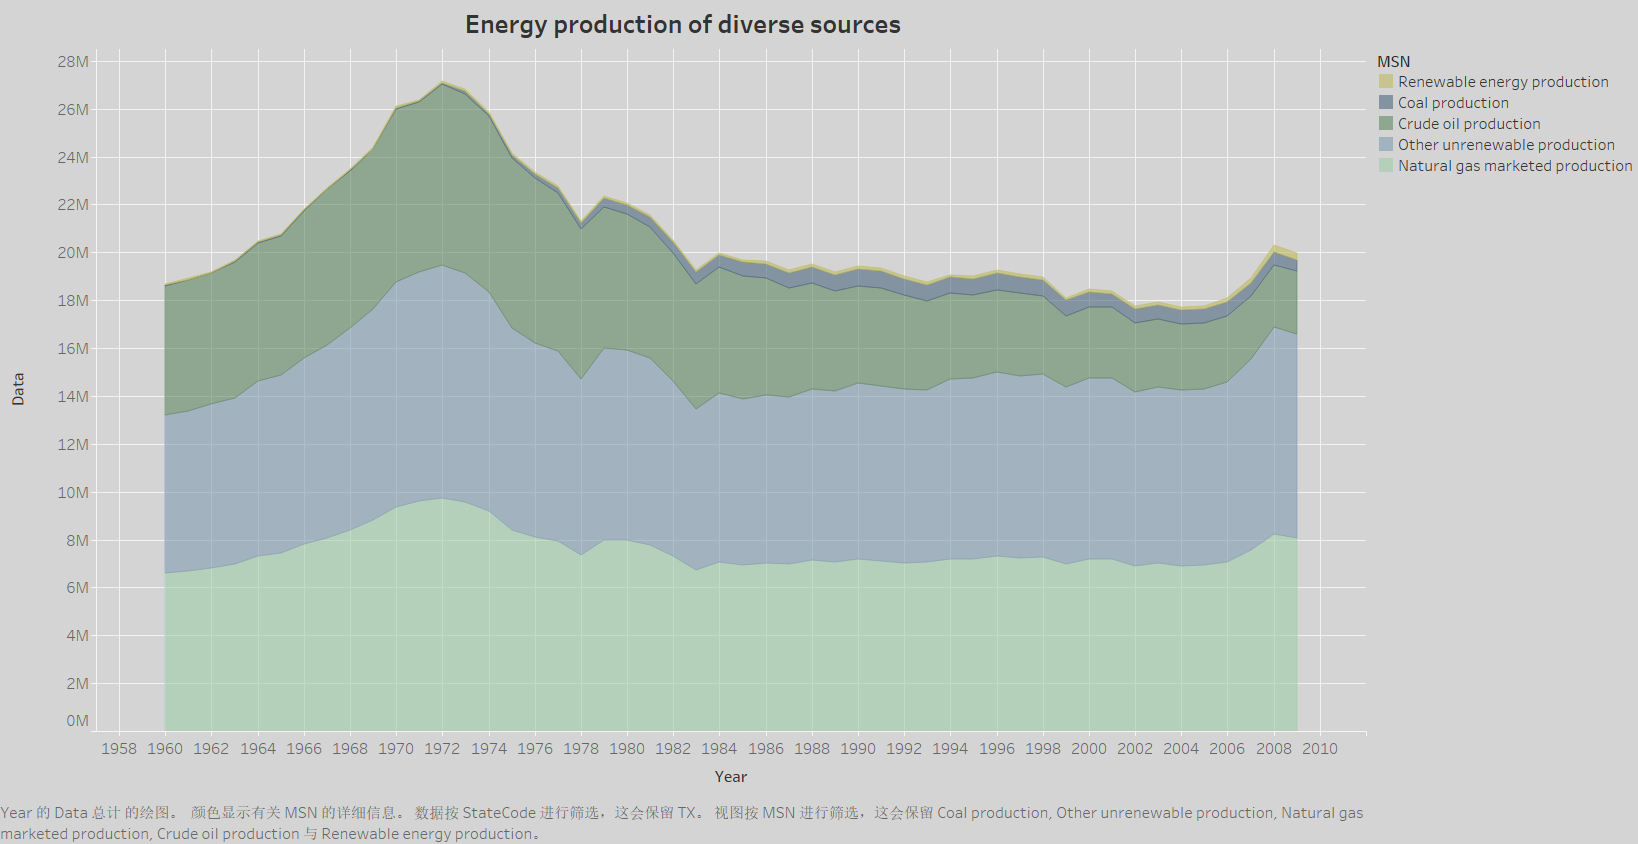
\includegraphics[width=0.313\textwidth]{ep/tx-2.png}}
\hspace{\fill}
   \subfloat[\label{ep-tx-3}]{%
      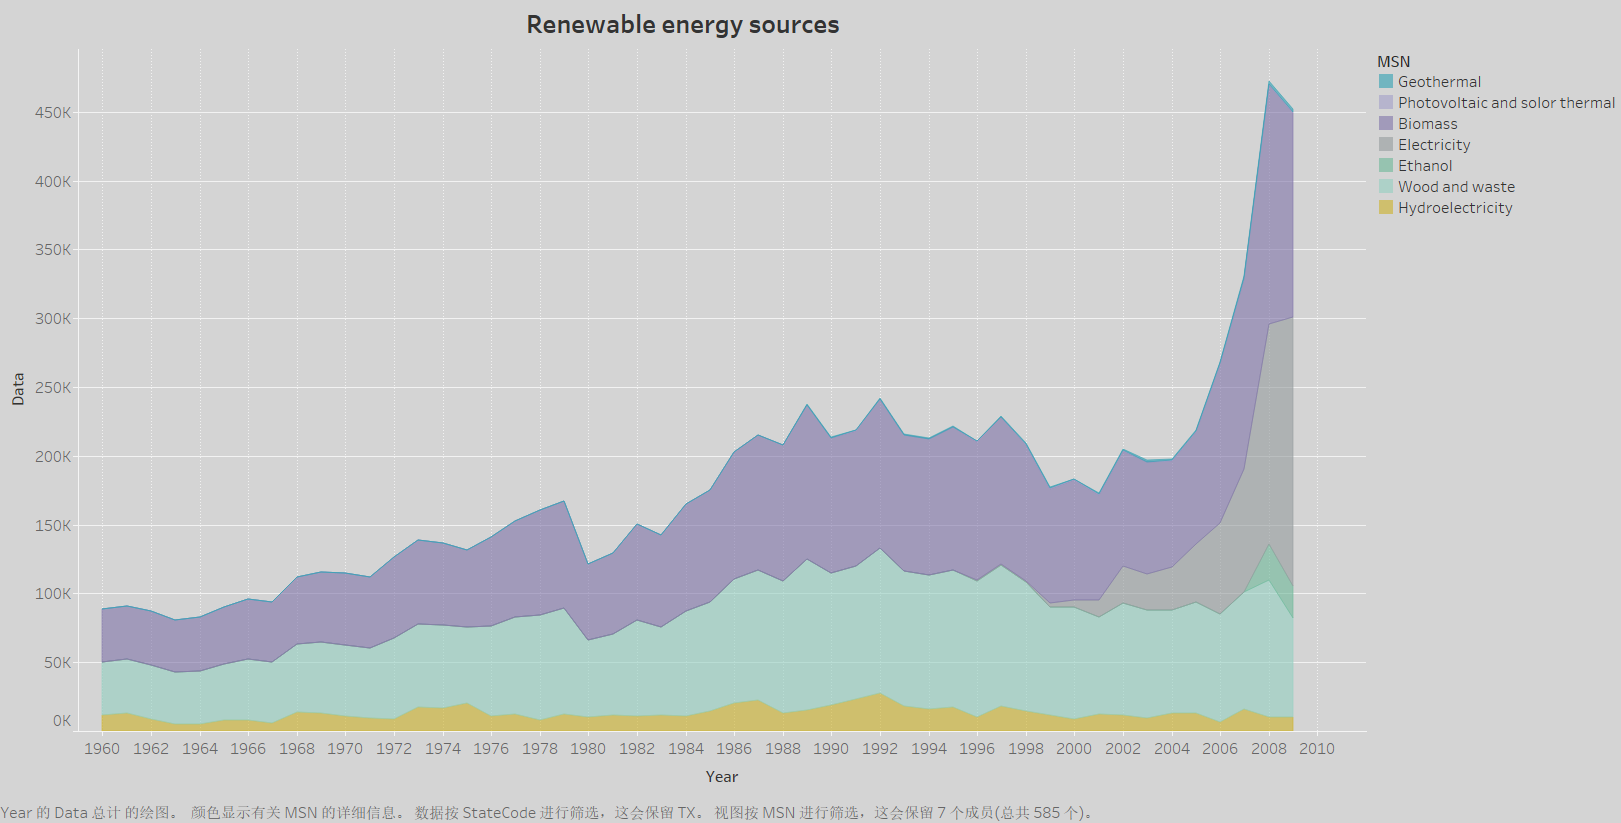
\includegraphics[width=0.32\textwidth]{ep/tx-3.png}}
    \caption{The energy profile for Texas (a) Energy consumption in diverse sectors (b) Energy production in diverse sources (c) Renewable energy usage}
    \label{fig:ep_tx}
\end{figure}

\section{XGBoost Modeling}
Our work is to find the relationship between types of main energy and $y$, which represents the energy consumption of the state.
Here we define $y$ as "total energy consumption per capita", and we hope to find the importance of each energy by fitting $y$ through the model.
Initially, we try to use liner-regression model such as general linear model and ridge regression to fit the $y$ and get the weights of every feature, but linear model doesn’t fit very well and the error is too large.
Then it occurs to us that we can use XGBoost Algorithm, which can fit $y$ well and output the importance of every feature.

\subsection{Introduction to XGBoost Algorithm}
XGBoost is an improvement of GBDT, which has been popular for many years.
The biggest difference between XGBoost and GBDT is its definition of the objective function~\eqref{eq:obj}:
\begin{equation}  \label{eq:obj}
Obj^{(t)} = \sum_{i=1}^{n} l\left( y_i, \hat{y}_i^{(t-1)} + f_t(x_i)\right) + \Omega (f_t) + constant
\end{equation}
where $l$ is the loss function, $\Omega$ is a regularization term which consists of two regularization terms, $L_1$ and $L_2$, and $constant$ is a constant term.

Applying Taylor's theorem~\eqref{eq:taylor}, we can get an approximation of the objective function~\eqref{eq:obj_appr}, which in this case only depends on the first and second derivative.
\begin{equation}  \label{eq:taylor}
f(x + \Delta x) \simeq f(x) + f'(x) \Delta x + \frac{1}{2} f''\Delta x^2
\end{equation} 
\begin{equation}  \label{eq:obj_appr}
Obj^{(t)} \simeq \sum_{i=1}^{n} \left[ l\left(y_i, \hat{y}_i^{(t-1)}\right) + g_i f_t\left(x_i\right) + \frac{1}{2} h_i f_t^2\left(x_i\right)\right] + \Omega (f_t) + constant
\end{equation}
where
\begin{equation}
g_i = \frac{\partial l(y_i, \hat{y}^{(t-1)})}{\partial \hat{y}^{(t-1)}},\quad h_i = \frac{\partial^2 l(y_i, \hat{y}^{(t-1)})}{{\left[\partial \hat{y}^{(t-1)}\right]}^2}
\end{equation}

Let's do a little refinement to the definition of $f$. Like GBDT, we will have some decision trees., but here the tree is split into the structure part $Q$ and the leaf weight part $w$.
The structure function $Q$ maps the input to the index number of the leaf, and $W$ gives the leaf score corresponding to each of the cable quotes.
Defining this complexity contains the number of nodes in a tree, and the $L_2$ modulus square of the output score on each tree leaf node.

Using this new definition, we can rewrite the objective function as follows, in which $I_j$ is defined as the set of samples on each leaf.

\begin{equation}
I_j = \left\{i | q(x_i) = j\right\}
\end{equation}

Here is the objective function, where $g$ is the first derivative, and $g$ is the second derivative.
\begin{IEEEeqnarray}{rCl}
Obj^{(t)} &\simeq& \sum_{i=1}^{n} \left[g_i f_t\left(x_i\right)
+ \frac{1}{2} h_i f_t^2\left(x_i\right)\right] + \Omega(f_t)\\
&=& \sum_{i=1}^{n} \left[g_i \omega_q\left(x_i\right) + \frac{1}{2} h_i \omega_q^2\left(x_i\right)\right]
+ \gamma T + \lambda \frac{1}{2} \sum_{j=1}^{T} \omega_j^2 \\
&=& \sum_{j=1}^{T} \left[(\sum_{i \in I_j}g_i)\omega_j + \frac{1}{2} (\sum_{i \in I_j}h_i + \lambda)\omega_j^2\right] + \gamma T
\end{IEEEeqnarray}

This goal contains $T$ independent single variable quadratic functions. We define
\begin{equation}
G_j = \sum_{i \in I_j}g_i
\end{equation}
\begin{equation}
H_j = \sum_{i \in I_j}h_i
\end{equation}

Finally we can get
\begin{IEEEeqnarray}{rCl}
Obj^{(t)} &=& \sum_{j=1}^{T} \left[(\sum_{i \in I_j}g_i)\omega_j + \frac{1}{2} (\sum_{i \in I_j}h_i + \lambda)\omega_j^2\right] + \gamma T \\
&=& \sum_{j=1}^{T} \left[G_j\omega_j+ \frac{1}{2} (H_j + \lambda)\omega_j^2\right] + \gamma T
\end{IEEEeqnarray}

Now, take the derivative of $w_j$ equal to $0$,
\begin{equation}
\omega_j^{*} = - \frac{\sum_{i \in I_j}g_i}{\sum_{i \in I_j}h_i + \lambda}
\end{equation}

and then add the optimal solution to the formula,
\begin{equation}
Obj = -\frac{1}{2}\sum_{j=1}{T}\frac{G_j^2}{H_j + \lambda} + \gamma T
\end{equation}

\subsection{Advantages and Parameter Adjustment}
Due to its boosting thought, XGBoost can fit the target accurately, and thanks to its bagging thought of feature selection, it can prevent overfitting to a certain extent. Also, it helps us to calculate the weights of features.
In addition to the difference of objective function, XGBoost has a C++ implementation of Gradient Boosting Machine.
The biggest feature of XGBoost is that it can automatically use CPU's multithreading to parallelism, which means performing many calculations at the same time. This improves the accuracy of the algorithm.
More importantly, XGBoost is a boosting algorithm, but it select the features randomly.
Consequently, it can avoid overfitting and tell us the importance of every features by multiple iterations.
Due to its high accuracy, the weights it gives are more efficient than other algorithm such as linear-regression, simple neural network and so on.

However, the parameters of XGBoost are hard to adjust, because it have so many parameters, for example, eta, tree max depth, to mention just a few.
We take 5000 iteration and the algorithm can finally converge, which also can produce less error.
To avoid overfitting, we choose a small number for tree max depth.
As for the percentage of subsample, we set 70 like other sets, and the results show that these parameters work.

\subsection{Modeling Process}
We select a bunch of features from the 605 MSNs, such as $CLTCB$ and $HYTCB$, from 1960 to 2009.
They form this a $50 \times 14$ matrix, it contains the most important information of energy use about the state from 1960 to 2009, including both unrenewable and renewable energy.
To get the weights, we define $TETPB$ as $y$.
According to XGBoost Algorithm, we create a model between different energy use and total energy consumption per capita.
The weights here can be explained as the influence of different energy types on energy consumption per capita.
In view of our target, the weights of XGBoost can be used to measure the importance of the energy.


After using XGBoost, we can get the importance of our features($w_j$), and we calculate the percentage of the importance, which we define as the features' weight.

Next, we define $W$ as $\sum_{i=1}^{14} w_i x_i$, which represents the state's energy use in that year.
After getting $w_i$, we just need to add $x$ into the formula and get $W$ of every year.

\subsection{Analysis}
From the result we find that, Arizona's total energy consumption per capita is mainly influenced by coal production, coal total consumption and residual fuel oil total consumption, whereas that of New Mexico is mainly influenced by coal production, natural gas total consumption and residual fuel oil consumption.
It's easy to see that these two states are similar, which both focus on coal and residual fuel oil.
Nonetheless, Arizona's coal total consumption is more important than natural gas total consumption.
Thus, compared to Arizona, New Mexico needs more natural gas but not coal.
On the other hand, Arizona uses more coal but also produce more coal.
When it comes to California, its total energy consumption per capita is mainly influenced by coal total consumption, fossil fuel total consumption and crude oil production.
Finally, Texas is mainly influenced by coal production, natural gas total consumption and natural gas marketed production.
Although they all influenced by coal, California is influenced by using coal but Texas is affected by producing lots of coal.
This means Texas and New Mexico can output coal to California and Arizona.
It's interesting to observe that Texas needs a lot of natural gas, but they also produce a large amount of natural gas, which can be seen in its natural gas marketed production.
California uses coal and fossil fuel but produce more crude oil, yet it can use crude oil to get more energy.

Adding $w$ to the formula $W = Xw$, we calculate the $W$ of 4 states from 1960 to 2009~\eqref{fig:states-energy-use}.
\begin{figure}[!h]
     \centering
     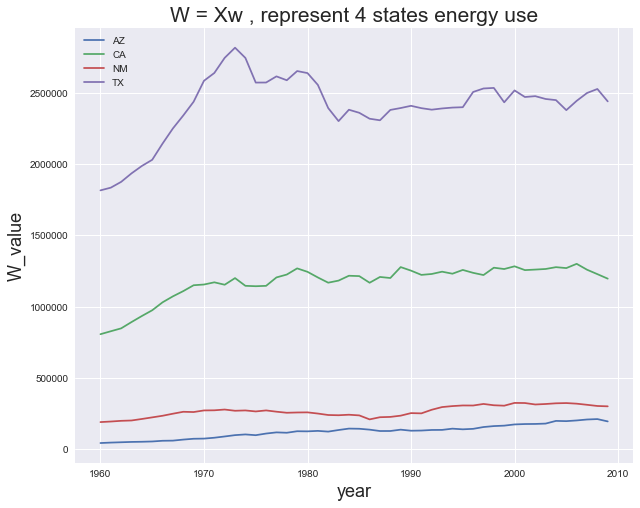
\includegraphics[width=0.5  \textwidth]{states-energy-use}
     \caption{Energy use of four states}
     \label{fig:states-energy-use}
\end{figure}

$W$ is the comprehensive use of energy, which is the weighted sum of some important unrenewable energy and renewable energy total consumption, so it's effective to define $W$ as the energy profile.
The picture~\ref{fig:states-energy-use} depicts the change of the energy profile about 4 states from 1960 to 2009.
From this picture, we can see that Texas uses the most energy and California ranks second.
New Mexico and Arizona use less energy and have no obvious difference.
Texas's energy use changes violently but others' changes more smoothly.

So we can see that, in terms of unrenewable energy, no matter production or consumption, coal influences the most on total energy consumption per capita, followed by fuel oil, fossil fuel and natural gas.
These energy are also very important, but as for other energy like motor gasoline, these states can use more renewable energy instead of these insignificant energy.
On the one hand renewable energy is cleaner, but on the other hand these energy influence less on total energy consumption per capita, so it's a good idea to increase the usage of renewable energy.

Closer observation reveals that some energy sources important to specific states, are not vital to the others however.
For example, asphalt and road oil total consumption ranks low in Texas but rank high in Arizona.
Fossil fuel total consumption ranks low in New Mexico but ranks high in California. Consequently, the four states can exchange the energy which is unimportant to them but vital to others according to the ranking picture above.
However, generally speaking, these states all need to increase renewable energy use to a certain extent.

\section{Predictions}
Based on our observation, the data appear to carry some seasonality. In order to model this characteristic properly, we use the Prophet forecasting model.

\subsection{Methodology}
The basic idea is shown is the following equation~\eqref{eq:comp}:
\begin{equation}  \label{eq:comp}
y(t) = g(t) + s(t) + h(t) + \epsilon_t
\end{equation}
where $g(t)$, $s(t)$ are trend functions representing the non-periodic and periodic changes respectively, $h(t)$ represents the effects of irregularly-scheduled events, and $\epsilon_t$ is the error term.

For $g(t)$, a piece-wise constant rate of growth provides a parsimonious and often useful model. Here the trend model is~\eqref{eq:linear}
\begin{equation}  \label{eq:linear}
g(t) = \left(k + a(t)^{T}\delta\right)t + \left(m + a(t)^{T}\gamma\right)
\end{equation}
where $k$ is the growth rate, $\delta$ has the rate adjustments, $m$ is the offset parameter,
and $\gamma_j$ is adjusted using automatic change-point selection to make the function continuous.


With the help of Fourier series~\eqref{eq:fourier}, we can construct a flexible model of periodic effects, or $s(t)$.
\begin{equation}  \label{eq:fourier}
s(t) = \sum_{n=1}^{N} \left(a_n \cos\left(\frac{2\pi nt}{P}\right) + b_n \sin\left(\frac{2\pi nt}{P}\right)\right)
\end{equation}

When it comes to $h(t)$, we are aware that events without a regular pattern such as El Niño and La Niña may have an impact on the data. However, due to the inherent unpredictability of future anomalies, we decide not to include them to our model.

\subsection{Application}
We use a standard Prophet forecasting model to model the trend of $W$.

As mentioned before, we detect a wave with a period of 25 years, which is presumably a result of the Kuznets swing, a medium-range economic wave with a period of 15–25 years connected with demographic processes. Taking this into consideration, we add a 25-year seasonality into the model.

\begin{figure}[!h]
   \subfloat[\label{w-prediction-az}]{%
      \includegraphics[width=0.5\textwidth]{w-prediction/az.png}}
\hspace{\fill}
   \subfloat[\label{w-prediction-ca}]{%
      \includegraphics[width=0.5\textwidth]{w-prediction/ca.png}}
\hspace{\fill}
   \subfloat[\label{w-prediction-nm}]{%
      \includegraphics[width=0.5\textwidth]{w-prediction/nm.png}}
\hspace{\fill}
   \subfloat[\label{w-prediction-tx}]{%
      \includegraphics[width=0.5\textwidth]{w-prediction/tx.png}}
    \caption{The prediction of $W$ in (a) AZ (b) CA (c) NM (d) TX }
    \label{fig:w-prediction}
\end{figure}

Here is the result. The blue line is the prediction of $W$ until the year 2050, and the light blue part marks its 95\% confidence interval. The energy profile of each state for 2025 and 2050 is listed below:

\begin{table}[h]
\centering
\begin{tabular}{rcccc}
& Arizona & California & New Mexico & Texas \\ \hline
2025 & 245620.8996 & 1293635.354 & 400980.219 & 2568748.067 \\
2050 & 313629.0864 & 1331776.615 & 484511.6994 & 2624274.833
\end{tabular}
\caption{The prediction of $W$ for 2025 and 2050}
\label{table:w-prediction}
\end{table}

\subsection{Validating the Model}
Time series cross validation is used to measure forecast error using historical data. We carried out a simulated historical forecast on $W$, where the model was fit to an initial history of thirty years, and a forecast was made on a one year horizon.

Here is the result.
\begin{table}[h]
\centering
\begin{tabular}{cccc}
Arizona & California & New Mexico & Texas \\ \hline
48.65\% & 54.05\% & 62.16\% & 32.43\%
\end{tabular}
\caption{Rate of correct predictions}
\label{table:w-cross-validation}
\end{table}

While it doesn't seem very impressive, note that we've merely used the data of the first 30 years, which only contains a single 25-year cycle. However, when making the prediction, all 50 data points are used, and the two complete 25-year cycle contained would hopefully make a big difference.


\section{Usage of Renewable Energy Sources}
We choose main renewable energy sources of four states and calculate what percentage each source takes up in the total.
It is worth mentioning that we get the production of fuel ethanol through a simple subtraction~\eqref{eq:calu-eth}, since there is no direct data concerning that.
\begin{equation}  \label{eq:calu-eth}
\text{Fuel Ethanol} = REPRB - ROPRB
\end{equation}
where $REPRB$ and $ROPRB$ stands for "Renewable energy production" and "Renewable energy production, other than fuel ethanol", respectively.

To compare the usage of renewable energy sources, we introduce several more variables.
$RenewP$ is a variable representing the proportion of renewable energy sources in the total energy production.
\begin{equation}
RenewP = \frac{REPRB}{TEPRB}
\end{equation}

The results are shown in the following tables.
\begin{table}[h]
\begin{tabularx}{\textwidth}{p{3.3cm}|XXXX}
& Arizona	& California & New Mexico & Texas \\ \hline
Hydroelectricity	& 62730.88 (50.59\%) & 272187.23 (31.65\%) & 2644.59 (5.17\%) & 10039.69 (2.22\%) \\ \hline
Geothermal energy & 329.09 (0.26\%) &127461.12 (14.82\%) & 317.06 (0.62\%) & 2057.02 (0.45\%) \\ \hline
Photovoltaic and solar energy & 4732.12 (3.81\%) & 31397.01 (3.65\%) & 282.52 (0.55\%) & 819.76 (0.18\%) \\ \hline
Electricity produced from wind & 288.35 (0.23\%) & 56996.57 (6.62\%) & 15095.96 (29.55\%) & 195454.76 (43.24\%) \\ \hline
Biomass & 35412.81 (28.56\%) & 224662.52 (26.13\%) & 17295.22 (33.85\%) & 148263.57 (32.80\%) \\ \hline
Wood and waste & 12867.29 (10.37\%) & 140159.17 (16.30\%) & 11633.20 (22.77\%) & 72108.45 (15.95\%) \\ \hline
Fuel ethanol & 7623.61 (6.14\%) & 6861.25 (0.79\%) & 3811.80 (7.462\%) & 23217.36 (5.13\%) \end{tabularx}
\caption{Major renewable energy resources in four states}
\label{table:name_1}
\end{table}
\begin{table}[h]
\begin{tabularx}{\textwidth}{p{4cm}|XXXX}
& Arizona	& California & New Mexico & Texas \\ \hline
Proportion of renewable energy resources & 14.17\% & 24.11\% & 1.24\% & 2.35\%
\end{tabularx}
\label{table:name_2}
\end{table}

As can be seen from the tables, each state has its own preference of using renewable energy resources, which may be affected by many factors like climate, geography, etc.

Here we give further discussion.

\begin{figure}[!h]
     \centering
     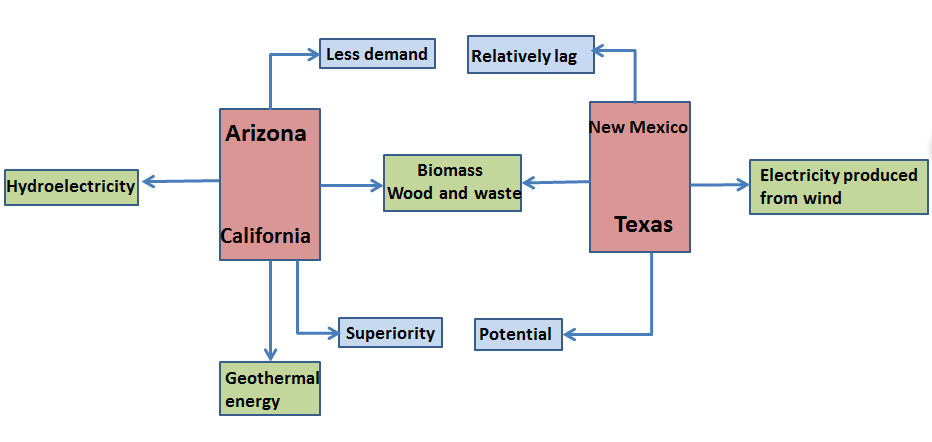
\includegraphics[width=0.9\textwidth]{comparison.png}
     \caption{Energy features of the four states}
     \label{fig:com}
\end{figure}

\begin{itemize}
\item \textbf{Arizona} \\
Arizona has relatively low demand for energy use, however, in which renewable energy resources takes a large proportion (shown in the energy profile for AZ), about 14.18\% in production, rankly only second to California.
Thus, we come to conclusion that Arizona has a good basis of exploiting and utilizing renewable energy resources. 
\item \textbf{California} \\
California has both the largest gross and the biggest proportion (24.11\%) of renewable energy resources usage, which indicates that California has already came to a relatively mature stage. 
\item \textbf{New Mexico} \\
Undoubtedly, the usage of renewable energy sources in New Mexico is not satisfying.
With great energy demand as California, New Mexico rarely make use of renewable ones.
Thus a "cleaner" energy profile is the most essential target for New Mexico.
\item \textbf{Texas} \\
Compared with other three states, Texas has enormous energy production and consumption.
With increasing proportion of renewable energy, Texas has the greatest potential of utilizing cleaner energy sources.
\end{itemize}

\subsection{Other Factors}

Now, we take geography, population, and climate into consideration.

\begin{table}[h]
\begin{tabularx}{\textwidth}{p{4cm}|XXXX}
& Arizona	& California & New Mexico & Texas \\ \hline
Population(million) & 6.93 & 39.25 & 2.08 & 27.86
\end{tabularx}
\caption{Population of the four states}
\label{table:name_4}
\end{table}

California has the largest population and the most advanced technology to utilize renewable energy resources.
Due to its location on the Pacific's "ring of fire" and because of tectonic plate conjunctions, California contains the largest amount of geothermal electric generation capacity in the United States.
As a result, California is the only state that make good use of geothermal energy. 

\begin{figure}[!h]
     \centering
     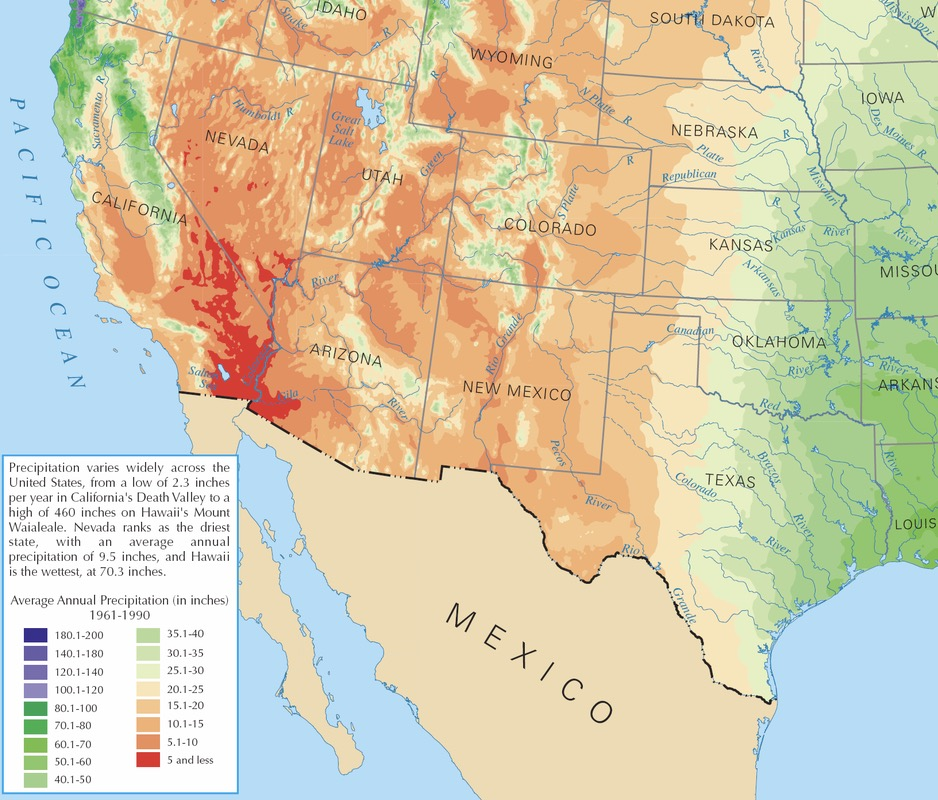
\includegraphics[width=0.5\textwidth]{map.jpg}
     \caption{A geographic map of the U.S.}
     \label{fig:geo}
\end{figure}

According to the geography, complex river networks are located in California and Arizona, making hydroelectricity a main source of renewable energy.
On the contrary, without many rivers in New Mexico, electricity produced from wind becomes the top priority due to its frequent gale.
However, as mentioned before, there is still a long way for New Mexico, since its production is still too low.

Last, with largest energy production and consumption, Texas also has every superiority to utilize varieties of renewable energy resources.
Up to now, wind power in Texas has achieved good results, standing at the top of four states in amount.
However, from the topographic map, we can see the river networks in Texas form favorable conditions for hydroelectricity.
Therefore, we want to hightlight that Texas has the greatest potential in usage of renewable energy sources.


\subsection{Which One is the Best? California}
Considering the utility of main renewable energy sources and its proportion it the gross, we use TPOSIS method to determine the best energy profile.

Firstly, we normalize the data matrix $A$ to get the decision matrix $B$.
The variables chosen are all benefit factors, so we adopt the same method below.
\begin{equation}
b_{ij} = \frac{a_{ij}}{\sqrt{\sum_{i=1}^{4}a_{ij}^2}}, i=1, 2, \dots, 4; j = 1, 2, \dots, 8
\end{equation}

Next, we form the normalized matrix $C$ with certain weight for each variable.
The weight is shown in the bubble diagram~\ref{fig:criteria}.

\begin{figure}[!h]
     \centering
     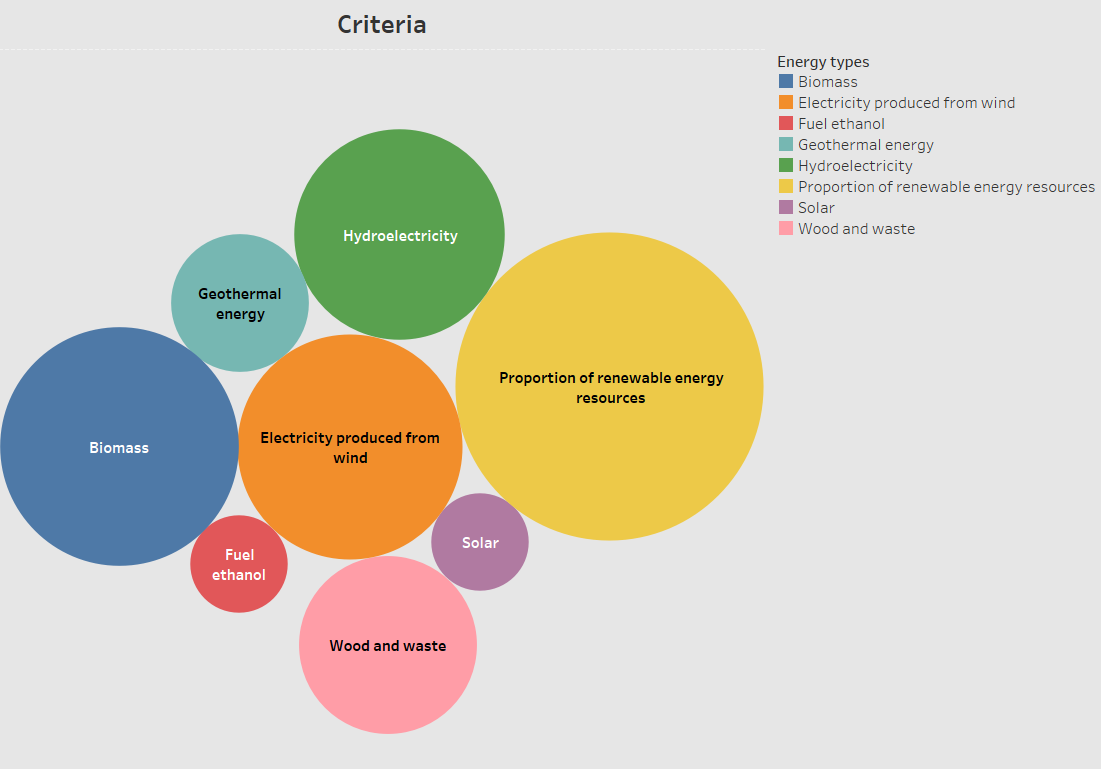
\includegraphics[width=0.7\textwidth]{criteria.png}
     \caption{Criteria}
     \label{fig:criteria}
\end{figure}

\begin{equation}
w  = \left[0.14\quad0.06\quad0.03\quad0.16\quad0.18\quad0.10\quad0.03\quad0.30\right]
\end{equation}
\begin{equation}
C_{ij} = w_i \times b_{ij}, i = 1, 2, \dots, 4
\end{equation}

Then we get the optimal solution and the negative ideal solution
\begin{equation}
C_i^{*} = \max_{i} C_{ij}, j = 1, 2, \dots, 8
\end{equation}
\begin{equation}
C_i^{0} = \min_{i} C_{ij}, j = 1, 2, \dots, 8
\end{equation}

Finally, we calculate the distance of each data list to the optimal solution and the negative ideal solution.

Distance to the optimal solution:
\begin{equation}
S_i^{*} = \sqrt{\sum_{j=1}^n(C_{ij} - C_{j}^{*})^2}, i = 1, 2, \dots, 4
\end{equation}

Distance to the negative ideal solution:
\begin{equation}
S_i^{0} = \sqrt{\sum_{j=1}^n(C_{ij} - C_{j}^{0})^2}, i = 1, 2, \dots, 4
\end{equation}

Integrated index:
\begin{equation}
f_i^{*} = \frac{S_i^{0}}{S_i^{0} + S_i^{*}}, i = 1, 2, \dots, 4
\end{equation}

\begin{table}[h]
\center
\begin{tabular}{c|cccc}
& Arizona & California & New Mexico & Texas \\ \hline
$s^{*}$ & 0.2635 & 0.1102 & 0.3534 & 0.2771 \\
$s^{0}$ & 0.1495 & 0.3262 & 0.0116 & 0.1817 \\
$f$ & 0.3619 & 0.7475 & 0.0318 & 0.3961 \\
rank & 3 & 1 & 4 & 2
\end{tabular}
\caption{The results of Topsis}
\label{table:name_3}
\end{table}

The result of our model clearly shows that \textbf{California} has the best energy profile.


\section{Prediction of Renewable Energy Usage Targets}

Our prediction of the $RETCB$ of 2025 and 2050 is shown in figure~\ref{fig:re-prediction} . The same technique is used as in the prediction of $W$.

\begin{figure}[!h]
   \subfloat[\label{re-prediction-az}]{%
      \includegraphics[width=0.5\textwidth]{re-prediction/az.png}}
\hspace{\fill}
   \subfloat[\label{re-prediction-ca}]{%
      \includegraphics[width=0.5\textwidth]{re-prediction/ca.png}}
\hspace{\fill}
   \subfloat[\label{re-prediction-nm}]{%
      \includegraphics[width=0.5\textwidth]{re-prediction/nm.png}}
\hspace{\fill}
   \subfloat[\label{re-prediction-tx}]{%
      \includegraphics[width=0.5\textwidth]{re-prediction/tx.png}}
\hspace{\fill}
    \caption{The prediction of $RETCB$ in (a) Arizona (b) California (c) New Mexico (d) Texas}
    \label{fig:re-prediction}
\end{figure}

As before, the blue line is the prediction of $W$ until the year 2050, and the light blue part marks its 95\% confidence interval. The prediction of renewable energy usage targets of each state for 2025 and 2050 is listed in table~\ref{table:re-prediction}:

\begin{table}[h]
\centering
\begin{tabular}{rcccc}
& Arizona & California & New Mexico & Texas \\ \hline
2025 & 128327.9859 & 963652.5339 & 18797.11625 & 212369.961 \\
2050 & 155304.4328 & 1199923.714 & 26812.56441 & 298504.3516
\end{tabular}
\caption{The prediction of $RETCB$ for 2025 and 2050}
\label{table:re-prediction}
\end{table}

\subsection{Validating the Model}
Table~\ref{table:re-cross-validation} shows the result of cross validation, using the same configuration as before.
\begin{table}[h]
\centering
\begin{tabular}{cccc}
Arizona & California & New Mexico & Texas \\ \hline
29.73\% & 70.27\% & 29.73\% & 43.24\%
\end{tabular}
\caption{Rate of correct predictions}
\label{table:re-cross-validation}
\end{table}

Again, for the same reason, we believe our prediction is better than what's shown in table~\ref{table:re-prediction}.

\section{Targets and Actions in the Compact}

\subsection{Goals}
Based on our comparison between the energy profile of each state, our criteria for the best profile, and our predictions, we mainly discuss the goals of renewable energy usage in three aspects.

\begin{enumerate}
\item Make energy profile of every state cleaner and more renewable
According to our results, the proportion of renewable energy usage is not ideal in all the four states, even California which has the best energy profile. Therefore, more utilization of cleaner energy should be included in the interstate compact. As each state has its own preponderance of using certain renewable energy, this goal coordinate with the following ones to some extent. The targets are listed below:
\begin{enumerate}
\item Increase the percentage that renewable energy takes in each state, California better more than 30\%, while others have dramatic improvements, especially New Mexico.
\item Substitute the most polluted energy resources gradually.
\item Exploit the great potential cleaner energy resources in Texas.
\end{enumerate}
\item Technological assistance from superior state to the ones lag behind
Among the four states, California is the most developed one with the largest population, of which the technology for utilizing renewable energy resources stands at the top. Therefore, California ought to contribute more to improve the skills of exploiting cleaner energy of other three states, especially Texas and New Mexico.
\item Energy redistribution to maximize its utility
To maximize the utility of energy usage, redistribution of energy sources is the best way, because some resources, not important to specific states, might be vital to other states. Therefore, the transportation of some certain energy from the states, that it ranks low, to those with high rank is a beneficial method. This goal can be achieved through the advice given below.
\end{enumerate}

\subsection{Recommended Actions}
\subsubsection{Arizona}
\begin{enumerate}
\item Exploit geothermal energy like California.
\item Make good use of photovoltaic and solar energy.
\item Export motor gasoline to Texas and California.
\item Develop renewable energy to replace motor gasoline.
\end{enumerate}

\subsubsection{Texas}
\begin{enumerate}
\item Exploit hydroelectricity and wind power.
\item Transmit electricity to other states in order to increase the demand.
\item Export asphalt and road oil to Arizona and New Mexico.
\item Decrease crude oil production and develop renewable energy.
\end{enumerate}

\subsubsection{California}
\begin{enumerate}
\item Provide technical assistance to other states, especially New Mexico and Texas.
\item Take its advantage of rich geothermal energy by making more use of it.
\item Decrease the consumption of environmentally unfriendly energy, and import cleaner energy from Texas and Arizona instead.
\item Exploit photovoltaic and solar energy.
\item Export residual fuel oil to other states, especially Arizona.
\item Decrease coal production and develop renewable energy.
\end{enumerate}

\subsubsection{New Mexico}
\begin{enumerate}
\item Change the energy structure gradually yet completely, by exporting more resources and importing technology of utilizing cleaner energy.
\item Exploit wind energy.
\item Export fossil fuel and motor gasoline to California
\item Export motor gasoline to Texas.
\item Develop renewable energy to replace motor gasoline and fuel fossil fuel.
\end{enumerate}



\newpage

\section{Memorandum}
\begin{DESCRIPTION}
\item [To] Governors
\item [From] Team \# 82104
\item [Date] \today
\item [Subject] Energy Production
\end{DESCRIPTION}

As of 2009, Arizona and California is doing fairly well in terms of energy profile, whereas New Mexico and Texas need some work. However, all of the four states depends greatly on fossil energy, which is not very clean.

According to our model, if no policy changes are made, the energy efficiency of all states will keep growing, though in a very slow rate and no without some serious fluctuating.
Coincidentally, the same result applies to the usage of renewable energy.
This is not bad, but we can do better with an energy compact.

we recommend the following goals for the compact.

\subsection*{Take Your Advantages}
States are suppose to use good of every natural resource they own.
For example, Texas may develop hydroelectricity and wind power more vigorously, since it's windy and full of river.

\subsection*{Exchange Material and/or Technology}
Some states are rich in natural resources but leak the technology to exploit it.
In this case, states with these technologies could consider providing technical assistance to them in exchange for their resources.
This would be a win-win deal for both side.

\subsection*{Think Ahead}
In the short run, conventional energy is more economical, since it's cheaper and yields more energy.
However, renewable energy can provide huge strategic advantages in the long run, most notably a cleaner environment and an energy source which will never be exhausted.


\newpage

\begin{thebibliography}{99}
\bibitem{1} Ümran Şengül, Miraç Eren, Seyedhadi Eslamian Shiraz, Volkan Gezder, Ahmet Bilal Şengül, Fuzzy TOPSIS method for ranking renewable energy supply systems in Turkey, Renewable Energy, Volume 75, 2015, Pages 617-625
\bibitem{2}Tianqi Chen and Carlos Guestrin. XGBoost: A Scalable Tree Boosting System. In 22nd SIGKDD Conference on Knowledge Discovery and Data Mining, 2016
\bibitem{3} Crude oil price forecasting using XGBoost,Published in: Computer Science and Engineering (UBMK), 2017 International Conference on, Date of Conference: 5-8 Oct. 2017
\bibitem{4} Taylor SJ, Letham B. (2017) Forecasting at scale. PeerJ Preprints 5:e3190v2 https://doi.org/10.7287/peerj.preprints.3190v2
\bibitem{5} \url{http://pbpython.com/prophet-overview.html}
\bibitem{6} \url{https://en.wikipedia.org/wiki/Kuznets_swing}
\end{thebibliography}

\begin{appendices}

\section{MATLAB Source Code}
\textbf{matlab.m}
\lstinputlisting[language=Matlab]{code/matlab.m}

\section{Python Source Code}
\textbf{model.py}
\lstinputlisting[language=Python]{code/model.py}

\textbf{W.py}
\lstinputlisting[language=Python]{code/W.py}

\textbf{MSN.py}
\lstinputlisting[language=Python]{code/MSN.py}

\textbf{RETCB.py}
\lstinputlisting[language=Python]{code/RETCB.py}



\end{appendices}
\end{document}

%% 
%% This work consists of these files mcmthesis.dtx,
%%                                   figures/ and
%%                                   code/,
%% and the derived files             mcmthesis.cls,
%%                                   mcmthesis-demo.tex,
%%                                   README,
%%                                   LICENSE,
%%                                   mcmthesis.pdf and
%%                                   mcmthesis-demo.pdf.
%%
%% End of file `mcmthesis-demo.tex'.
